\subsection{Revving the VIPUR approach to expand rare disease diagnostics}
	\subsubsection{Preparatory steps for using the VIPUR approach}
		After the publication of VIPUR the tools, data and applications became available at the open science framework (OSF) \cite{} which were downloaded and reviewed. All applications from the Rosetta software suite (Section \ref{subsec:MM_Rosetta}) were pre-compiled without support for MPI (Section \ref{subsec:MM_MPI}) and with that not the ability to benefit from multiple CPUs. The Rosetta software suite was rebuilt with MPI support in a slurm job where the compilation could benefit from multiple CPU cores.
	\label{subsubsec:RES_Prepare}
	
	\subsubsection{VIPUR resolving system incompatibilities}
	Within the VIPUR pipeline residues were mutated to determine the effects of a structural mutation, by default missense mutations were inserted with PyMOL (Section \ref{subsec:MM_PyMOL}), an alternative method integrated within the pipeline for situations wherein PyMOL was not accessible Pyrosetta (Section \ref{subsec:MM_PyRosetta}) could be used. Neither of these programs could be built or compiled because the lack of Open graphics library (OpenGL) for PyMOL and having the incorrect C++ and C libraries for PyRosetta. To bypass both programs and still be able to introduce mutations into PDB files Modeller (Secton \ref{subsec:MM_Modeller}) was introduced and built.
	
	\begin{figure}[!ht]
		\centering
		\begin{subfigure}{0.45\textwidth}
			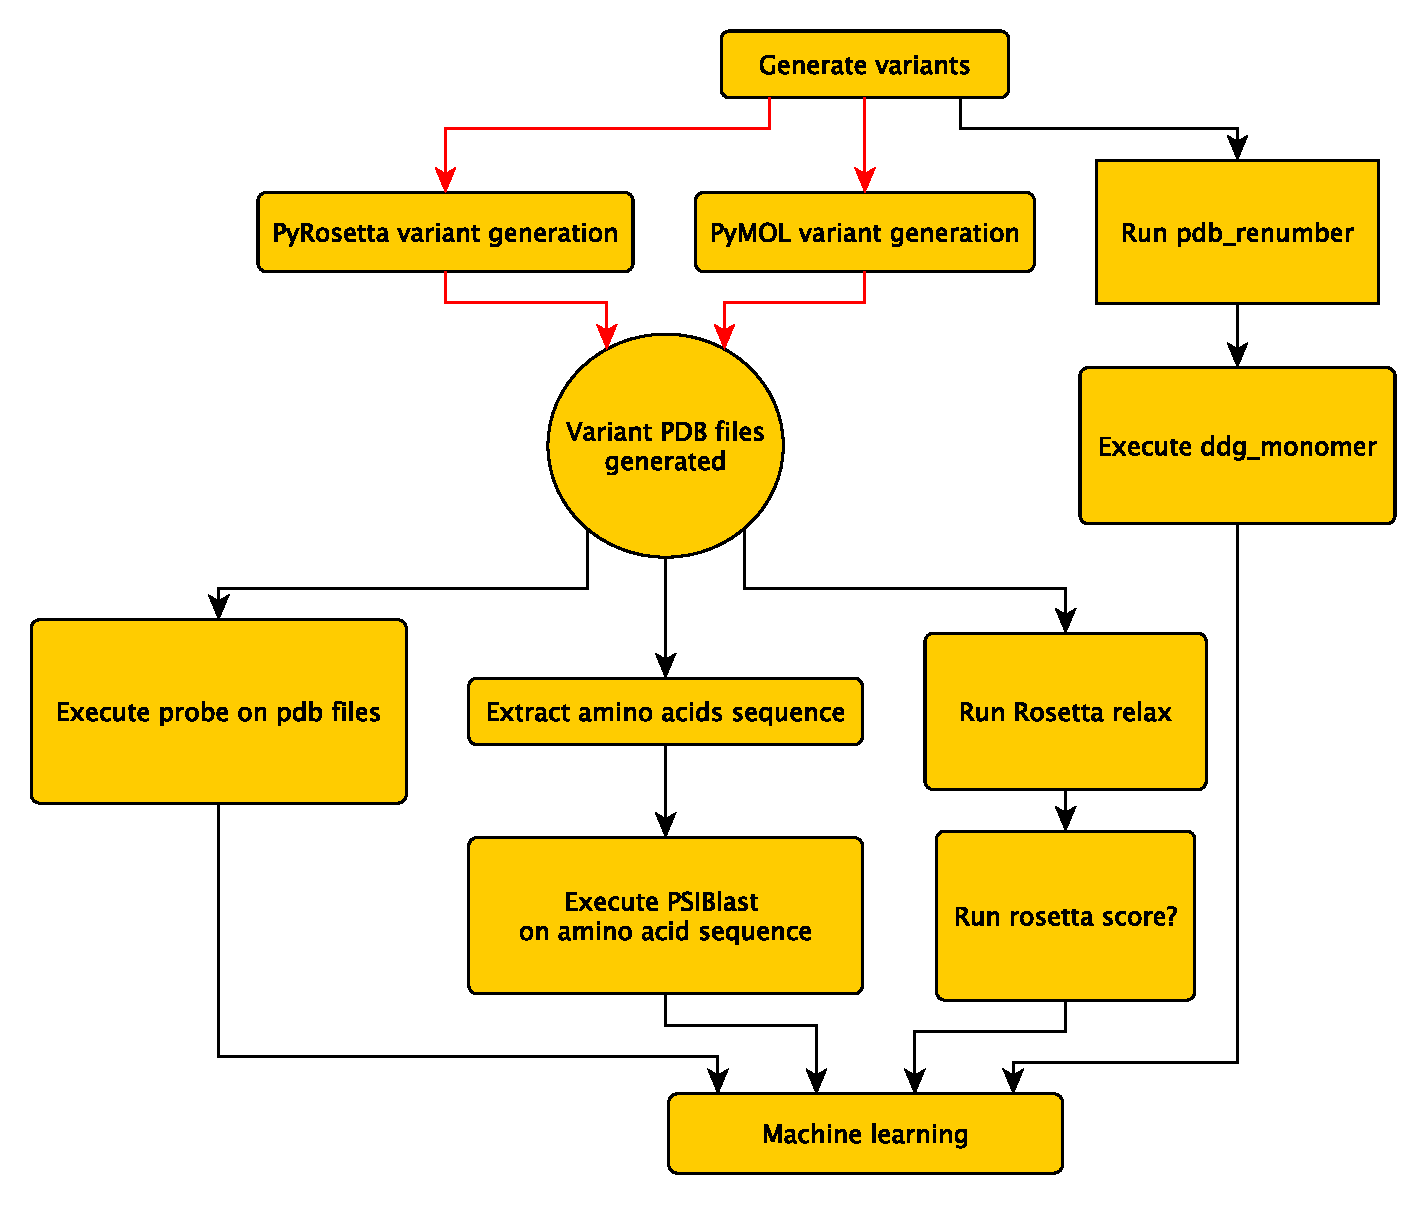
\includegraphics[width=\textwidth]{Flowcharts/VIPUR_approach.pdf}{a}
			\phantomcaption
			\label{fig:RES_VIPUR_approach}
		\end{subfigure}
		\begin{subfigure}{0.45\textwidth}
			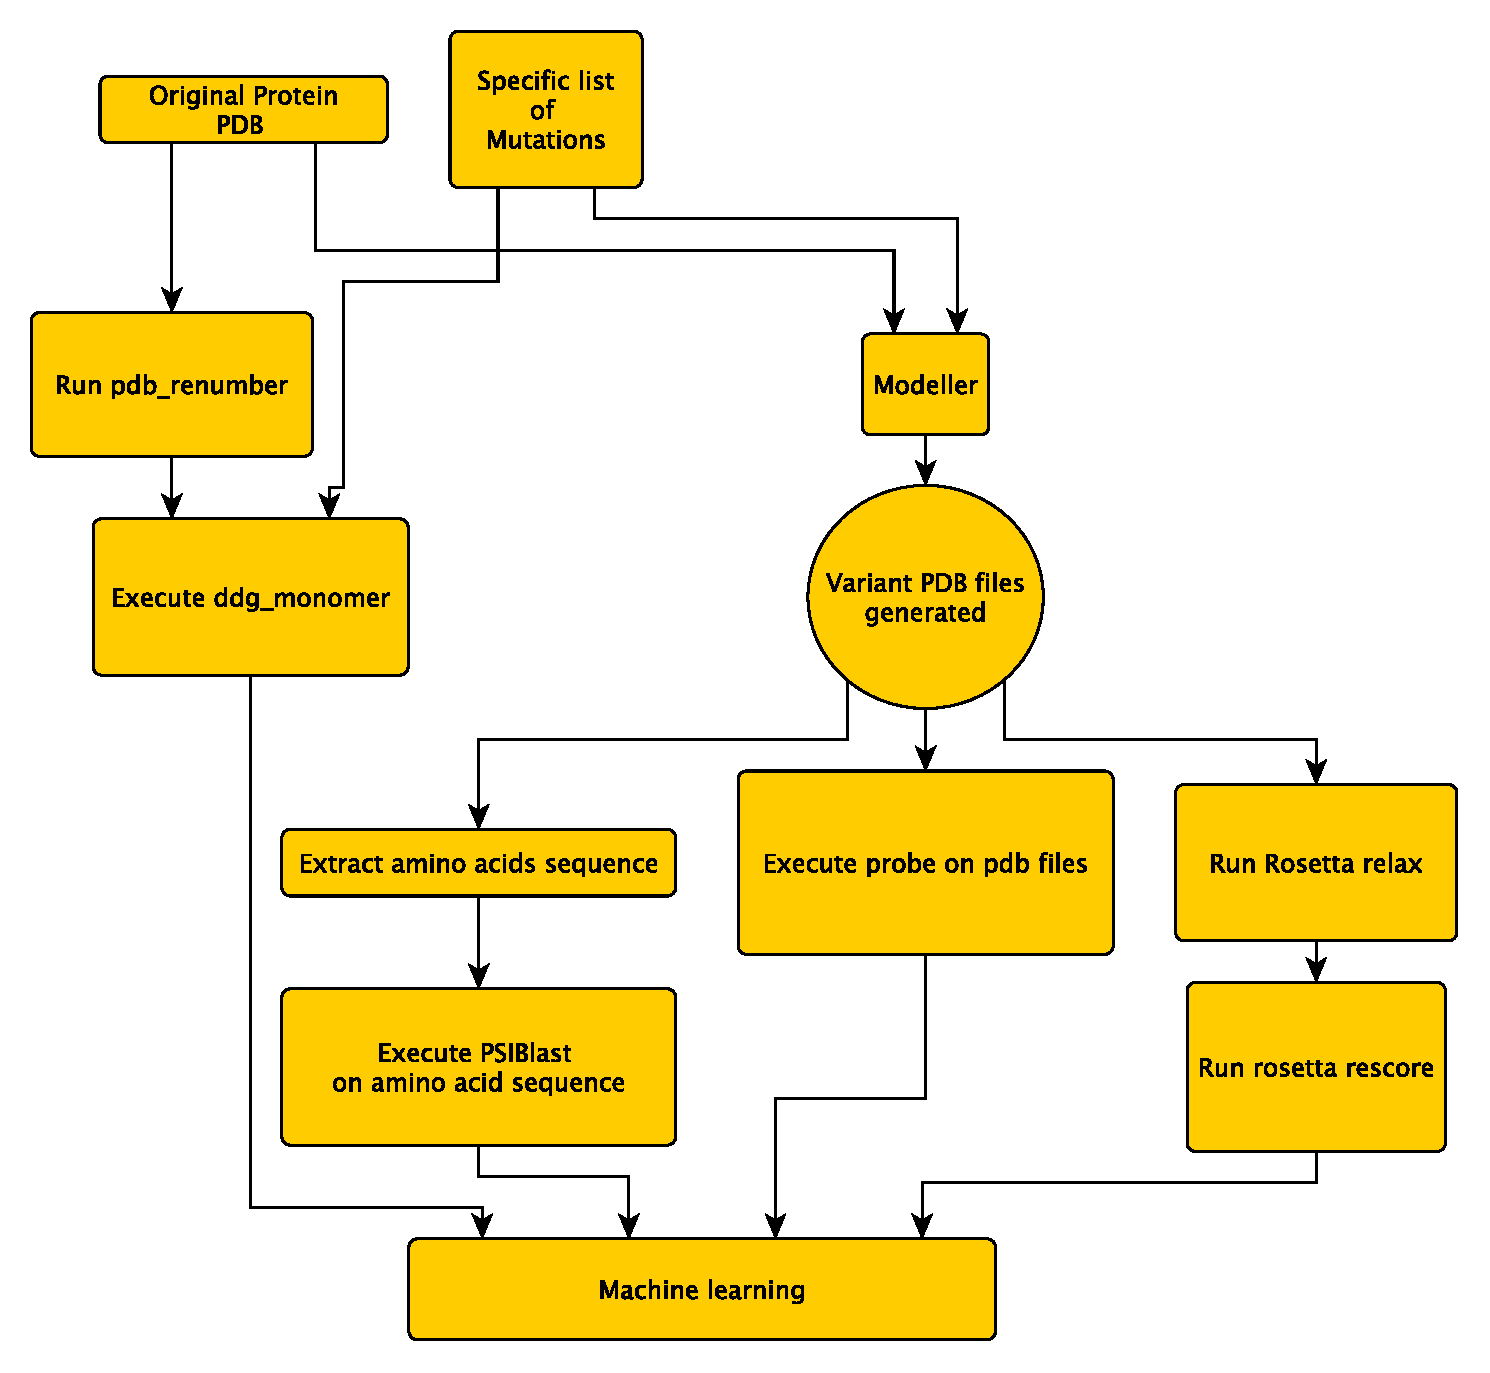
\includegraphics[width=\textwidth]{Flowcharts/Altered_VIPUR_approach.pdf}{b}
			\phantomcaption
			\label{fig:RES_Altered_VIPUR_approach}
		\end{subfigure}
		\caption[Flowcharts VIPUR pipeline and altered VIPUR pipeline]{Both flowcharts illustrate the VIPUR pipeline wherein each block is a procedure the central circle is the purpose of the mutated applications and each arrow represents the path to it. Figure \ref{fig:RES_VIPUR_approach} has red arrows that indicate that both methods were incapable to produce the mutated PDB files. Within figure \ref{fig:RES_Altered_VIPUR_approach} the alternative method is proposed wherein PyMOL and PyRosetta (Sections \ref{subsec:MM_PyMOL}, \ref{subsec:MM_PyRosetta}) is substituted by Modeller (Section \ref{subsec:MM_Modeller}) to acquire the mutated protein structures.}

		\label{fig:Flowcharts_of_old_and_altered_VIPUR}
	\end{figure}
	\label{subsubsec:RES_Incompatibility}
	\newpage
	
	\subsubsection{Expanding the VIPUR training set with data from TNFRSF1A by homology modeling and protein threading}
	Since the VTS did not have any features of TNFRSF1A (Section \ref{subsec:CD_TNFRSF1A}) the amino acid sequence was collected from Uniprot (Section \ref{subsec:MM_Uniprot}) and the protein from RCSB (Section \ref{subsec:MM_RCSB}). The structures available of TNFRSF1A were incomplete, fragments for the TNF $\alpha$ and $\beta$ binding site \cite{} were available and its death domain that interacts with TRADD \cite{} which plays a role in apoptosis (Section \ref{subsec:CD_TNFRSF1A}). To acquire a monomeric structure of TNFRSF1A two ab initio modeling web services I-TASSER and Robetta (Sections \ref{subsec:MM_I_TASSER}, \ref{subsec:MM_Robetta}) had been employed. Both were given the task to model the whole protein with and without a template to determine how well they could model a known structure and what it would form. Determination of which the best model was is based on the shortest distance ,defined root mean square deviation (RMSD), between a produced model compared to the X-ray crystallographic model of the TNFRSF1A binding site .
	
%	Solution structure of the tumor necrosis factor receptor-1 death domain, Sukits
	\begin{figure}[!ht]
		\centering
		\begin{subfigure}{0.45\textwidth}
			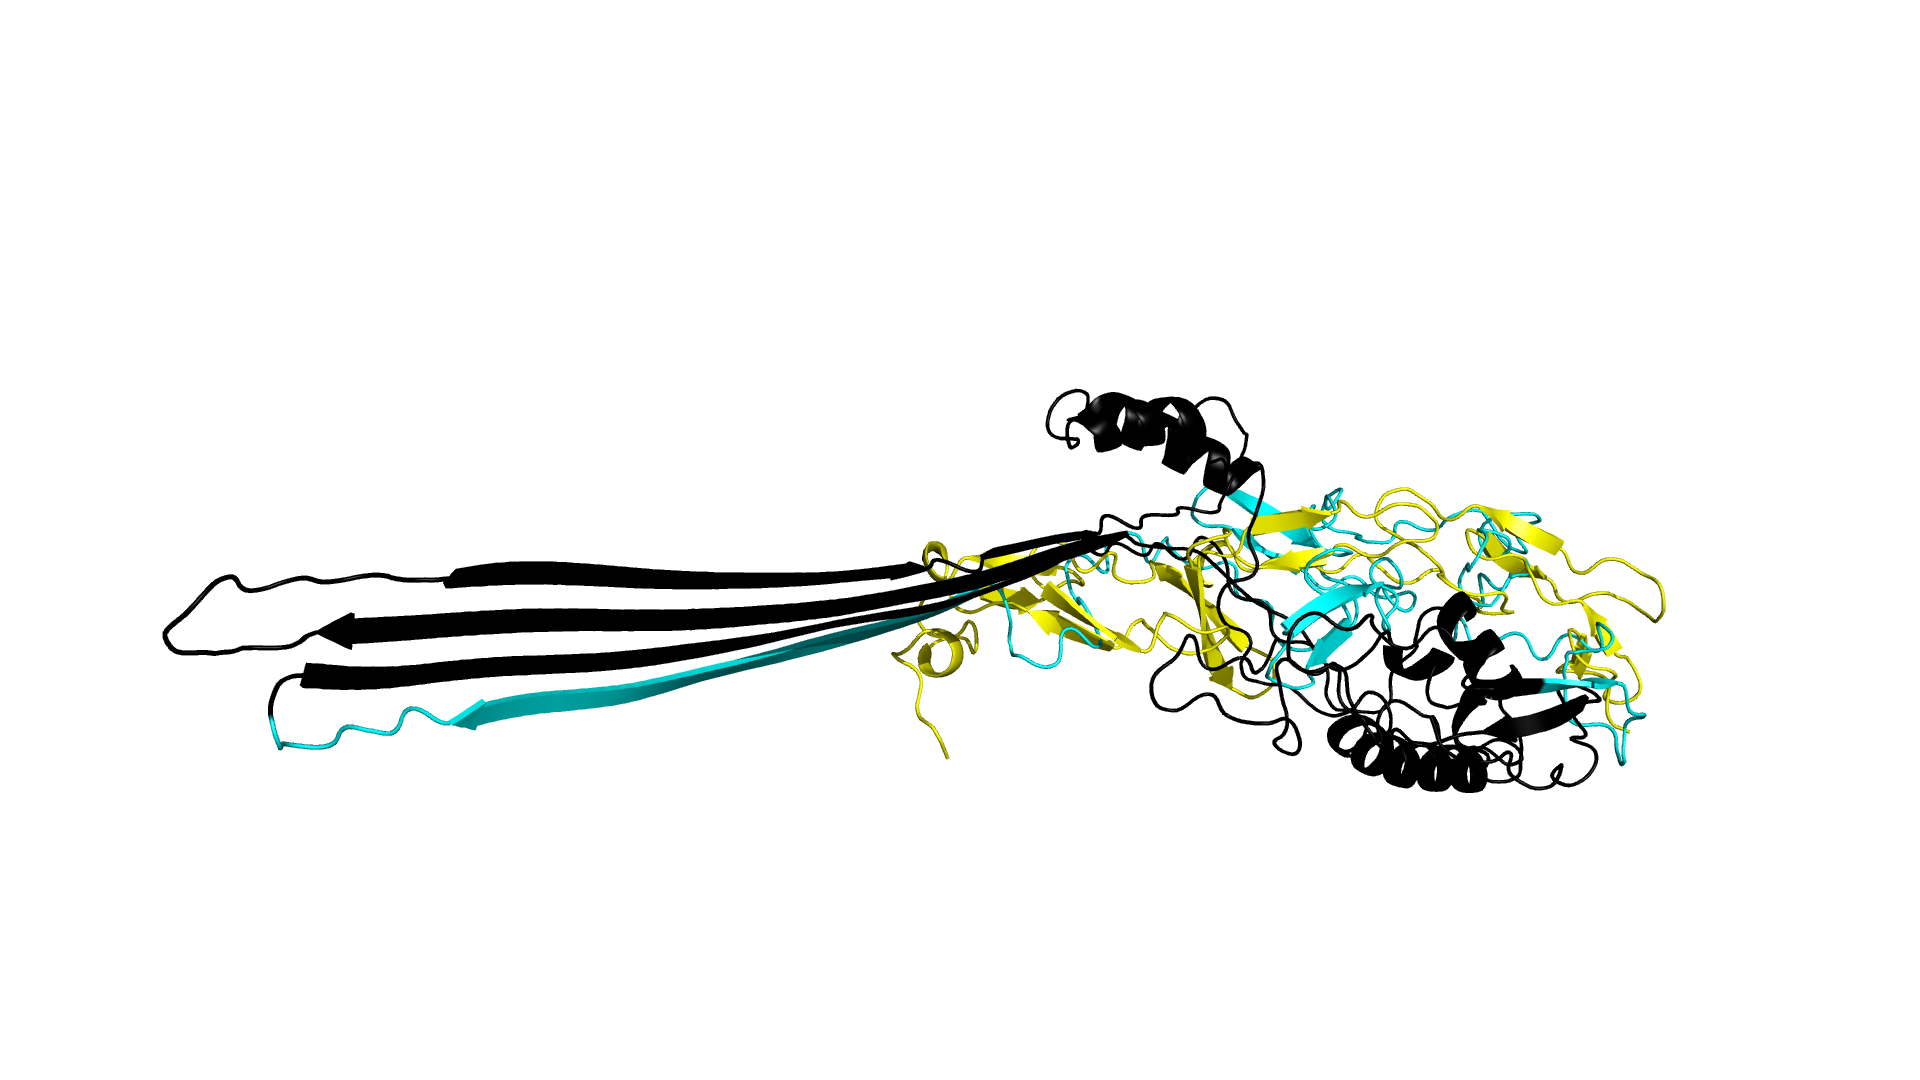
\includegraphics[width=\textwidth]{I_TASSER_Robetta_Images/1_EXT_ALIGN_I_TAS_WITHOUT_TEMPLATE.png}{a}
			\caption{RMSD = 28.786}
			\label{fig:RES_I_TASSER_Without}
		\end{subfigure}
		\begin{subfigure}{0.45\textwidth}
			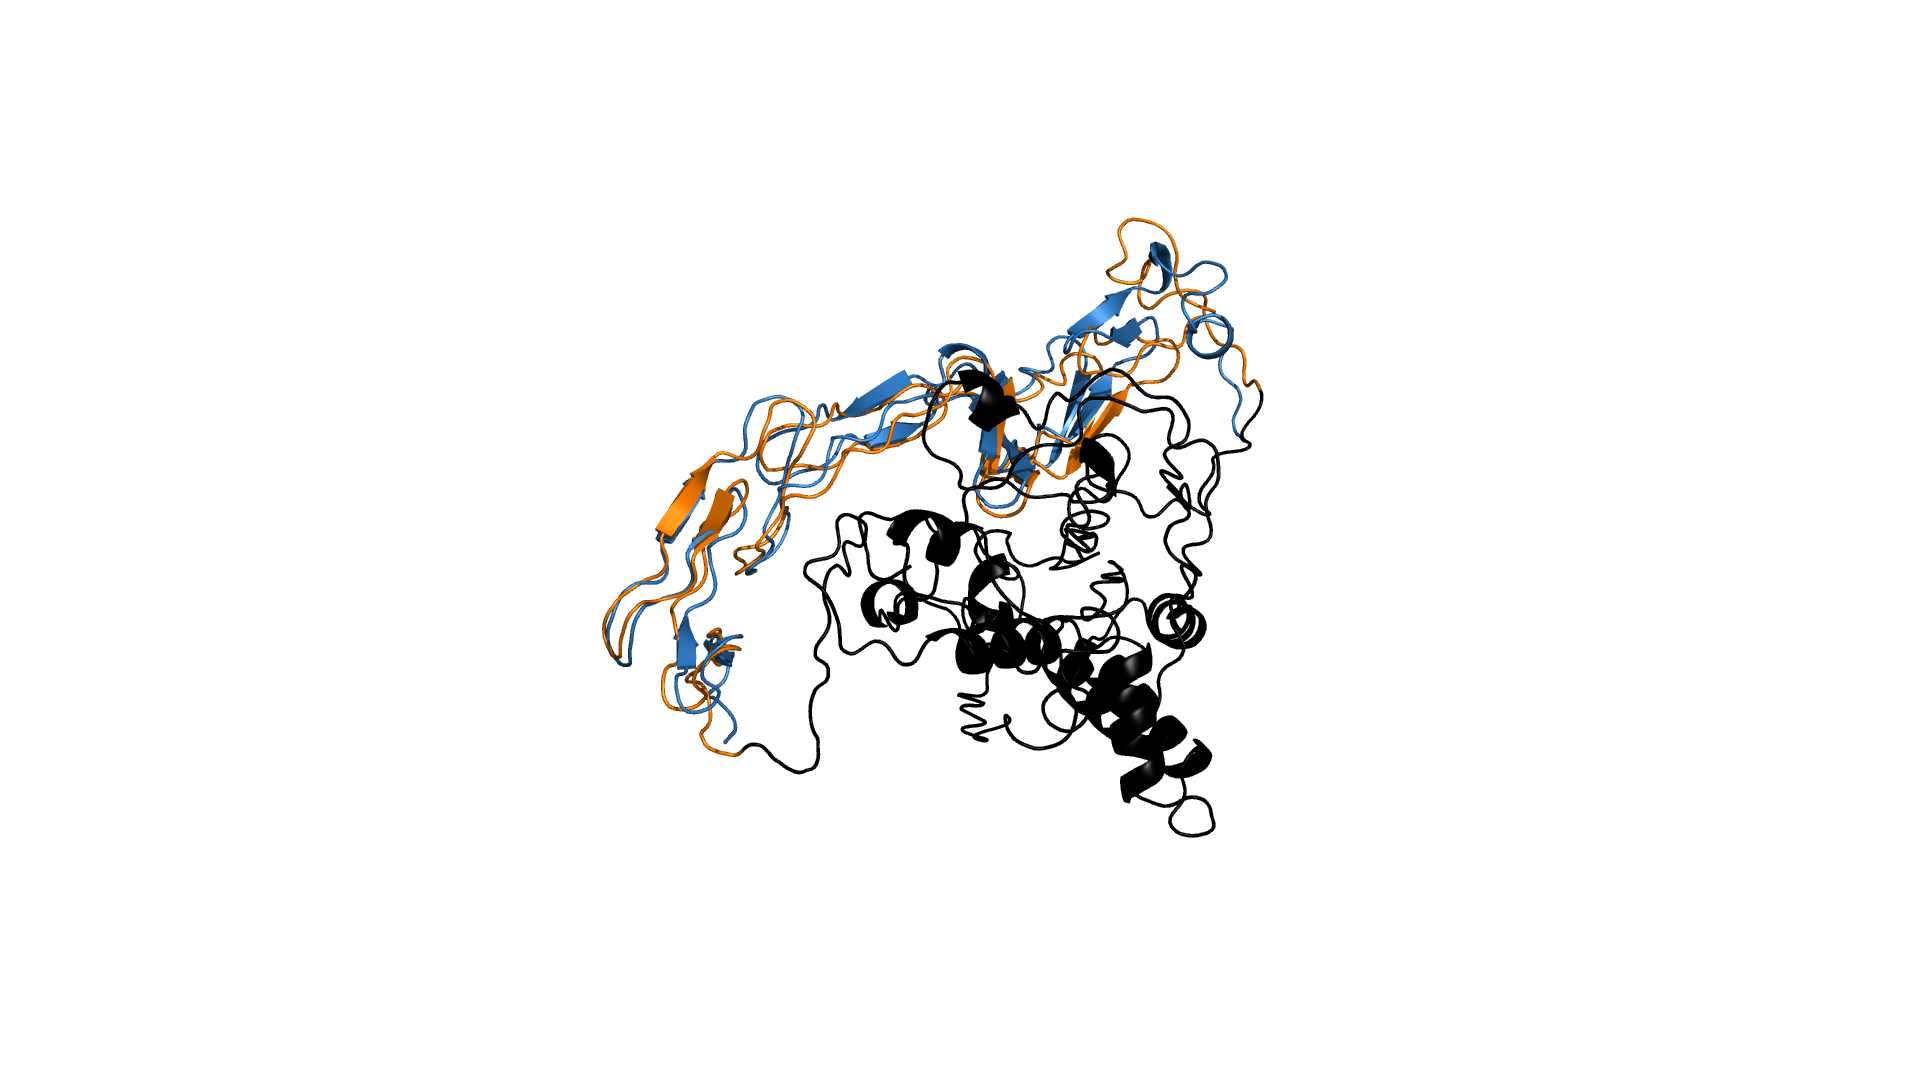
\includegraphics[width=\textwidth]{I_TASSER_Robetta_Images/1_EXT_ALIGN_I_TAS_WITH_TEMPLATE.png}{b}
			\caption{RMSD =  3.830}
			\label{fig:RES_I_TASSER_With}
		\end{subfigure}
		\begin{subfigure}{0.45\textwidth}
			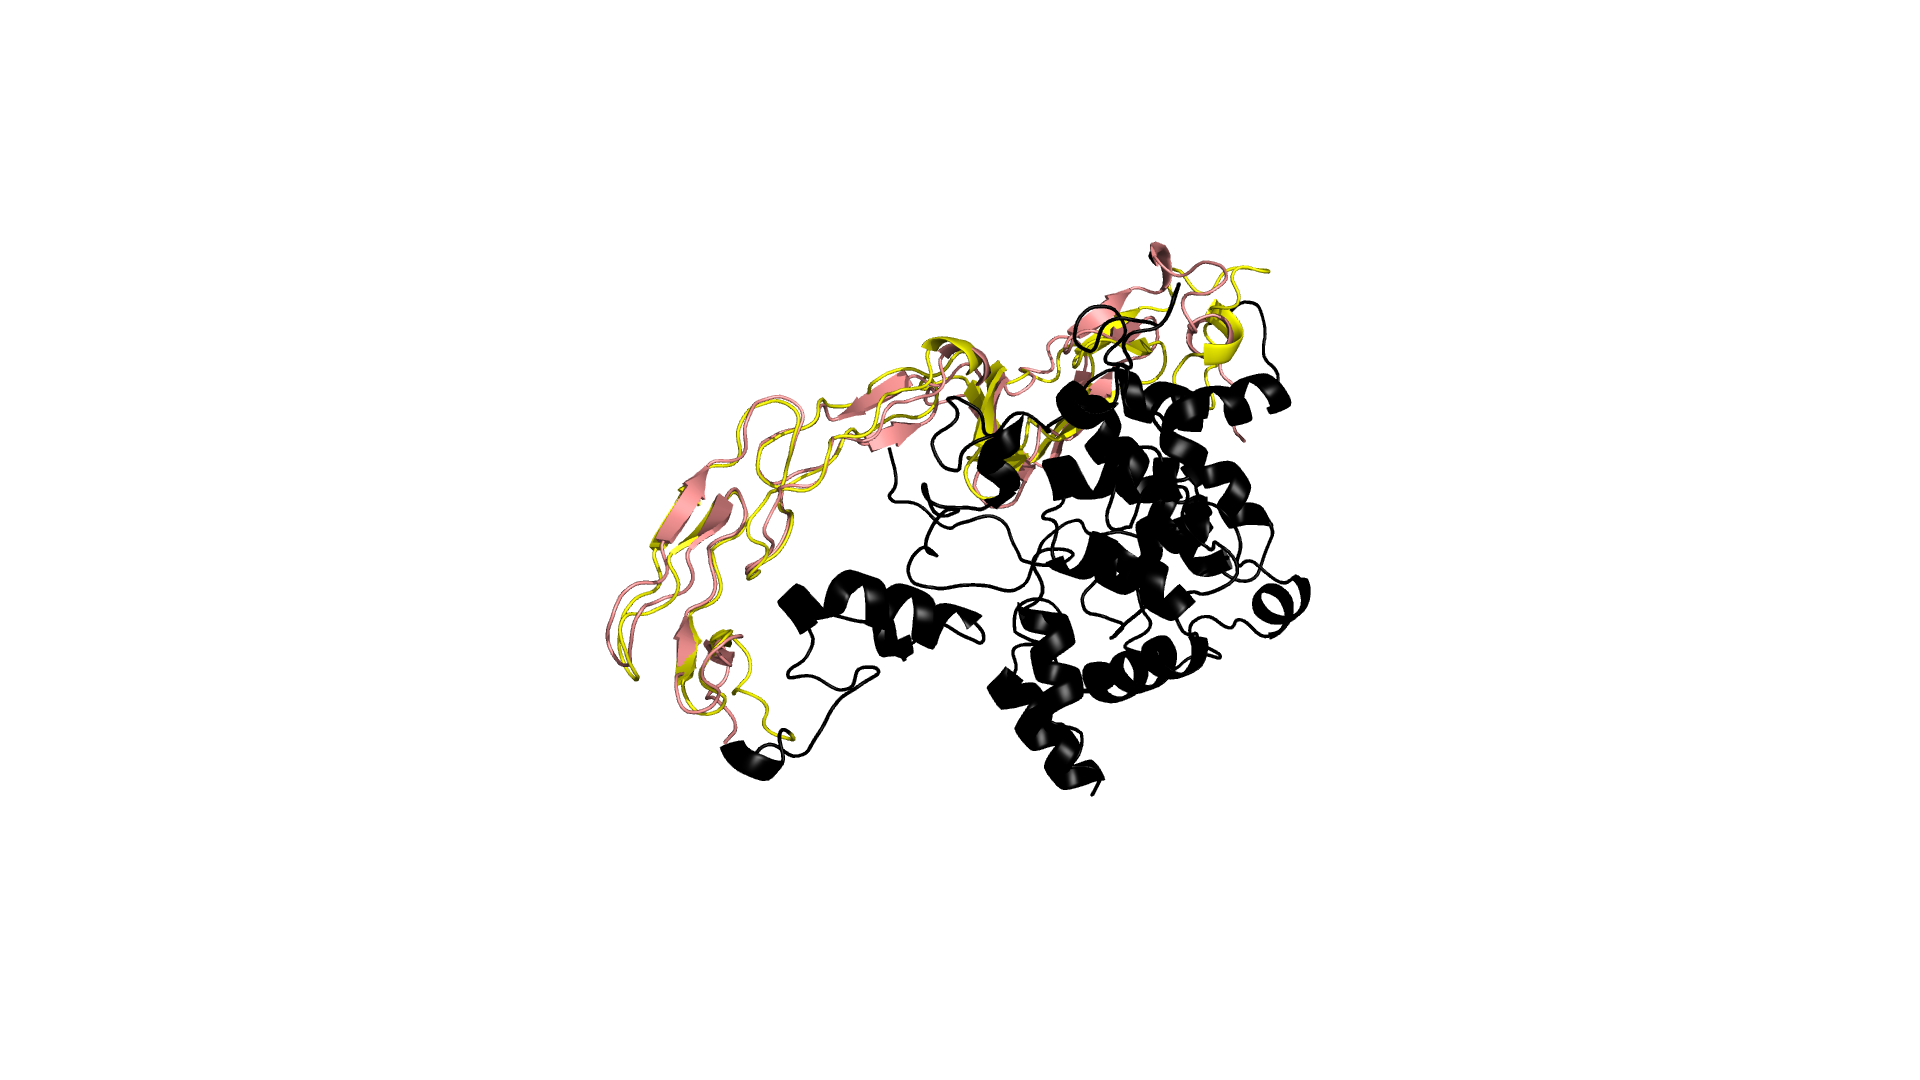
\includegraphics[width=\textwidth]{I_TASSER_Robetta_Images/1_EXT_ALIGN_ROB_WITHOUT_TEMPLATE.png}{c}
			\caption{RMSD =  3.067}
			\label{fig:RES_Robetta_Without}
		\end{subfigure}
		\begin{subfigure}{0.45\textwidth}
			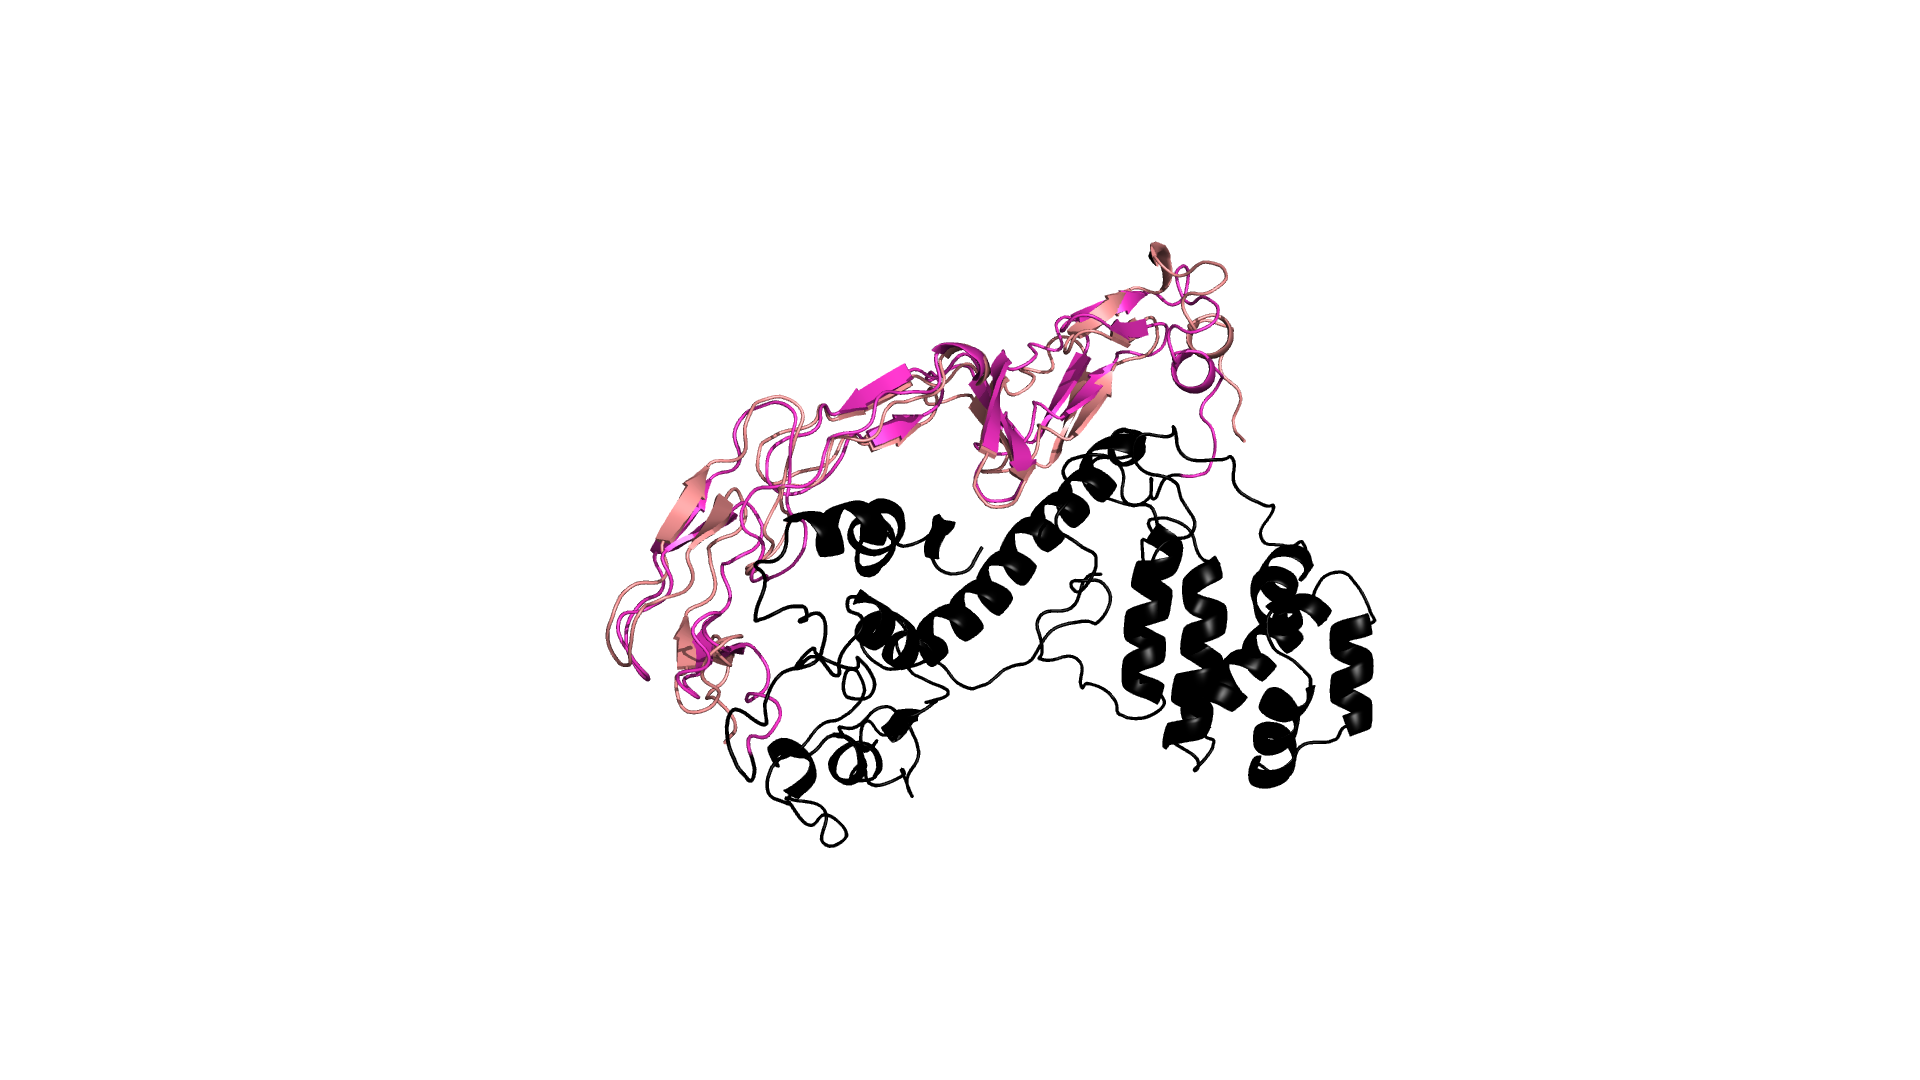
\includegraphics[width=\textwidth]{I_TASSER_Robetta_Images/1_EXT_ALIGN_ROB_WITH_TEMPLATE.png}{d}
			\caption{RMSD =  2.877}
			\label{fig:RES_Robetta_With}
		\end{subfigure}
		\caption[I-TASSER and Robetta models with and without templates]{3D structures of TNFRSF1A ( \ref{fig:RES_I_TASSER_Without}, \ref{fig:RES_I_TASSER_With}: I-TASSER, \ref{fig:RES_Robetta_Without}, \ref{fig:RES_Robetta_With}: Robetta) without (left: \ref{fig:RES_I_TASSER_Without}, \ref{fig:RES_Robetta_Without}) and with templates (right: \ref{fig:RES_I_TASSER_With}, \ref{fig:RES_Robetta_With}). The sky blue colored structure in each figure is an X-ray crystallographic model (1EXT) of the binding site of TNFRSF1A and the orange structure is the representation of that identical fragment in the model made by the web services.}
	\end{figure}
	\label{subsubsec:RES_Expanding_Models}

\newpage
\subsection{Analyses of proteins variants TNFRSF1A}
	\subsubsection{Requirements for determining structural and binding effects of protein variants}
	Currently there is no protocol available to asses protein variants with structural information, 
	
	Assessing protein variants and its effects can be the most informative when assessed from multiple fields of view, however this is out of scope for this project and to simplify the problem it brought down to the perspective of function an form.
	
	Function determines how certain parts of the protein behave within an environment and determine its effects on a pathway. In context with TNFRSF1A one part resides on the cell surface where it binds ligands and on the cytoplasmic side it can interact with protein that triggers an inflammatory response or apoptosis. When a mutation is introduced at the cell surface side it might not be able to form dimer formations that interact with TNF ligands or during transformation with the binding of TNF it is unable to bind trimers. 
	
	Wherein the perspective of form the deciding factors are the amino acid sequence and where it resides within the cell.
	
	A different perspective is form wherein the amino acid sequence determines how a protein structure will be formed.
	
%	Assessing protein variants and its effects should be studied with a multidisciplinary view wherein form and function are assessed. Within the aspect of form should be seen how a protein is formed
%	
%	
%	However due to difficulties with experiments it can be hard to unravel all the effects that can be caused by mutations.
%	
%	 A part of this view is to know what function the protein has before its mutated to determine its effect on a pathway or function. 
%	
%	How does the 
%	
%	
%%	 Effect
%	Can a cell or pathway still function without this protein? or is there an alternative mechanism within the cell that is less efficient in performing similar role? 
	
	\subsubsection{Tools for assessing protein variant mutation}
	Before introducing mutations it is helpful to know if they are observed since not every mutation has the same occurrence, therefore three tables with observed TNFRSF1A mutations(Sections \ref{subsec:MM_GAVIN_data_table}, \ref{subsec:MM_GnomAD}, \ref{subsec:MM_Infevers}) have been combined into a single table consisting of two columns. The first column contains strings that describe the: original residue, position and where the residue is mutated to, the second column describes the observed effect of the mutation.	
	\begin{table}[ht]
		\begin{tabular}{ l | l | l | l}
			Original residue & Position in the protein sequence & New residue & Classification\\ \hline
			Cys & 44 & Tyr & PATHOGENIC\\
			Thr & 44 & Pro & PATHOGENIC\\
			Thr & 44 & Ser & PATHOGENIC\\
		\end{tabular}
		\caption[Sample of combined tables with observed mutations]{The format wherein mutations were filtered from the GAVIN, GenomAD and Infevers tables (Sections \ref{subsec:MM_GAVIN_data_table},  \ref{subsec:MM_GenomAD}, \ref{subsec:MM_Infevers}), the first column is split into original residue within a structure the position where it resides in amino acid sequence and the residue where it is altered to.  In the last part with the available classifications: Benign Pathogenic, Likely Benign, Likely Pathogenic, Population, Uncertain significance (VOUS) and Na. To see the whole table visit the supplementary.}
		\label{table:Res_Filtered_Mutations}
	\end{table}
	
%	the function of the mutated protein is within a pathway 
%	A broad perspective should be taken with a 
%	To determine the effects of mutated residue awithin a protein variant a b than structural information should
%	Up until VIPUR and the development of similar approaches that benefit from structural information
%VIPUR: Variant Interpretation and Prediction Using Rosetta, Baugh



%Something about that we tried to use the VTS and add our protein for information.

%
%\begin{table}[ht]
%	\begin{tabular}{ l | l | l | l | l}
%		Iteration number & Filename & Chain & Residue index in chain & New residue\\ \hline
%		34 & 1tnr3\_TNFA & R & 0 & TYR\\
%		34 & 1tnr3\_TNFA & T & 0 & TYR\\
%		34 & 1tnr3\_TNFA & S & 0 & TYR\\
%		35 & 1tnr3\_TNFA & R & 0 & PRO\\
%		35 & 1tnr3\_TNFA & T & 0 & PRO\\
%		35 & 1tnr3\_TNFA & S & 0 & PRO\\
%		36 & 1tnr3\_TNFA & R & 0 & SER\\
%		36 & 1tnr3\_TNFA & T & 0 & SER\\
%		36 & 1tnr3\_TNFA & S & 0 & SER\\
%	\end{tabular}
%	\caption{The format that describes the mutations that should be made by Modeller (Section \ref{subsec:MM_Modeller}). The iteration number states if a mutation must be made in a single variant or in a different protein. Filename describes the protein to which the mutations are applied. Since structures can consist of multiple chains it has to be specified together with the index starting at 0 instead of 1 and finally to which residue it will be transformed.}
%		\label{table:Res_Modeller_Mutation_Format}
%\end{table}

